\documentclass[12pt]{exam}
\usepackage[utf8]{inputenc}
\usepackage[swedish]{babel}
\usepackage{enumitem}
\usepackage{graphicx}

\pagestyle{headandfoot}
\header{\footnotesize Klass:\\Namn:}{\Large\textbf{Organisk kemi}\medskip}{\footnotesize Naturkunskap 2 - 2025}
\headrule
\footrule
\setlength{\columnsep}{0.25cm}
\footer{}{Sida \thepage}{Organisk kemi}

\begin{document}

\section*{Instruktioner}
Provet består av frågor av olika typer. Läs frågorna ordentligt innan du svarar.

\subsection*{Poäng}
Antalet poäng är markerat för varje fråga. Totalt \textbf{22 poäng}.\\ \textit{För godkänt krävs minst 10 poäng.}

\vspace{5mm}
\hrule

\begin{questions}

\question Ange vilka partiklar en atom består av och vilken laddning de har. (\textbf{1 poäng})
\vspace{20mm}

\question Förklara följande ord: (\textbf{1 poäng})
\begin{itemize}
  \item grundämne
  \item atomnummer
  \item masstal
\end{itemize}
\vspace{5mm}

\question Hur många valenselektroner har syre? Motivera utifrån bilden. (\textbf{1 poäng})

\begin{figure}[h]
  \centering
  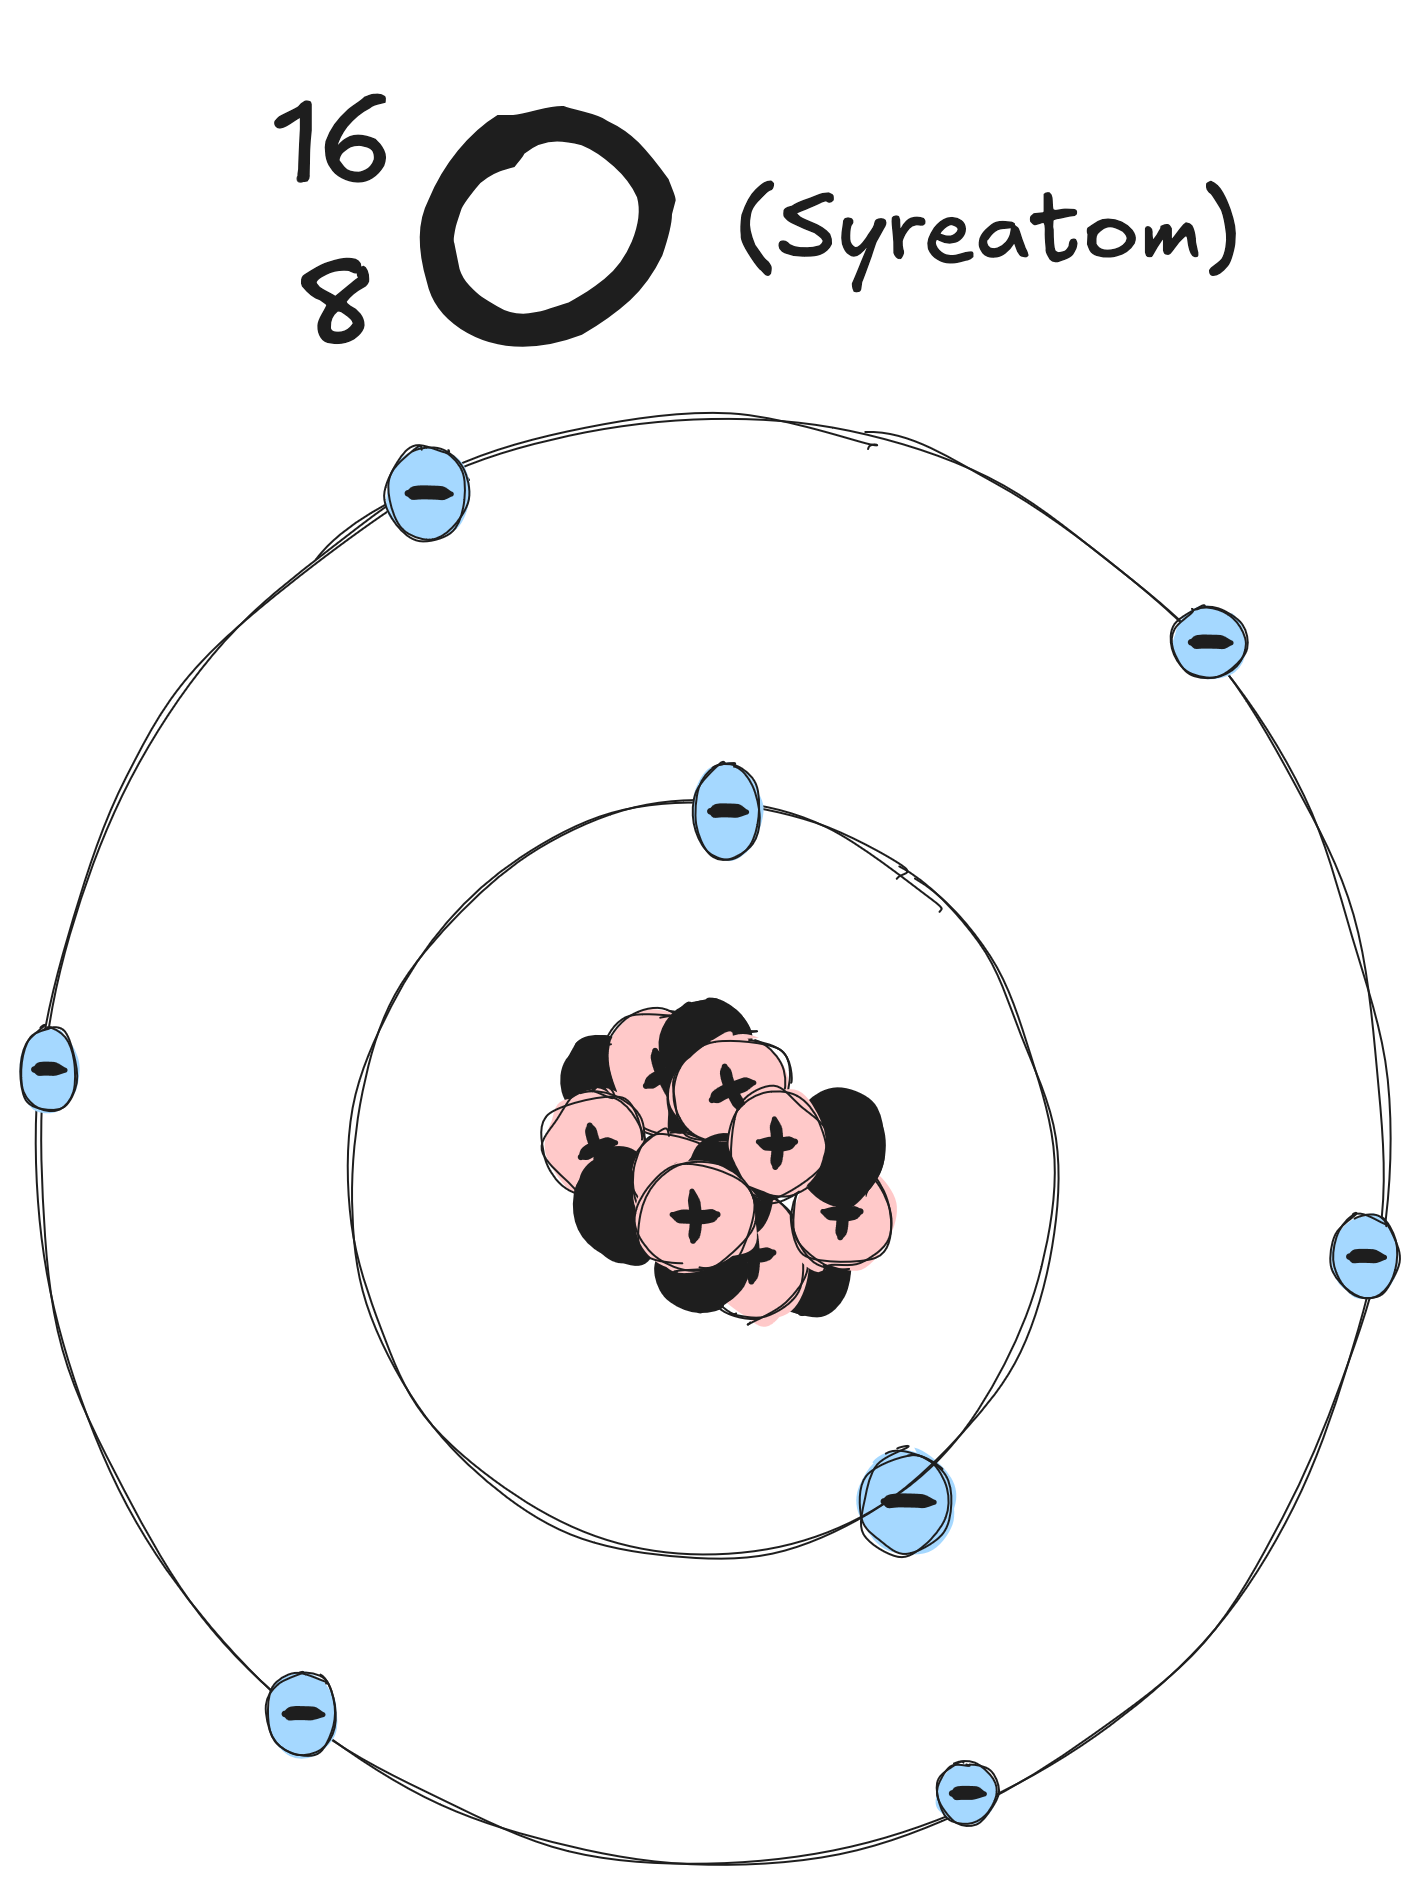
\includegraphics[width=0.25\textwidth]{syre-atom.png}
\end{figure}
\break

\question Vilka av följande molekyler ingår i \textbf{metan-serien}? (\textbf{1 poäng})
\begin{checkboxes}
  \choice Etan
  \choice Eten
  \choice Butyn
  \choice Propanol
  \choice Pentan
  \choice Glycerol
\end{checkboxes}
\vspace{5mm}

\question Vad är metanol och vad i dess kemiska struktur gör att det tillhör gruppen? (\textbf{2 poäng})
\vspace{20mm}

\question Vad är \textbf{polyeten} och hur är den uppbyggd? (\textbf{1 poäng})
\vspace{20mm}

\question Ge exempel eller förklara följande: (\textbf{2 poäng})
\begin{itemize}
  \item en monosackarid:
  \vspace{5mm}
  \item en disackarid:
  \vspace{5mm}
  \item stärkelse:
  \vspace{5mm}
  \item protein:
\end{itemize}
\vspace{5mm}

\question Vad kallas fettsyror som saknar dubbelbindningar? (\textbf{1 poäng})

\break

\question Ange om följande påståenden är sanna eller falska. (\textbf{2 poäng})
\begin{itemize}
  \item De flesta miljögifter är biologiskt nedbrytbara.
  \item Mikroplaster kan tas upp av djurplankton i haven.
  \item Miljögifter är ofta fettlösliga.
  \item De flesta miljögifter förekommer naturligt i höga koncentrationer i naturen.
  \item Koncentrationen av miljögifter är högre i toppkonsumenter än i producenter.
  \item Plaster bryts snabbt ner i naturen.
  \item Plaster kan bidra till spridning av miljögifter i naturen.
  \item Cocktail-effekten innebär att blandningar av kemikalier alltid är ofarliga.
\end{itemize}
\vspace{10mm}

\question Vad händer med kokpunkten för ett \textbf{kolväte} när det blir längre? (\textbf{1 poäng})
\begin{checkboxes}
  \choice Kokpunkten blir längre.
  \choice Kokpunkten blir kortare.
  \choice Kokpunkten förblir oförändrad.
\end{checkboxes}
\vspace{5mm}  

\question Hur påverkas \textit{struktur- och summaformel} hos \textbf{hexan} om det skulle omvandlas till \textbf{hexen} eller \textbf{hexyn}? Utgå från bilden på hexan nedan. (\textbf{2 poäng})

\begin{figure}[h]
  \centering
  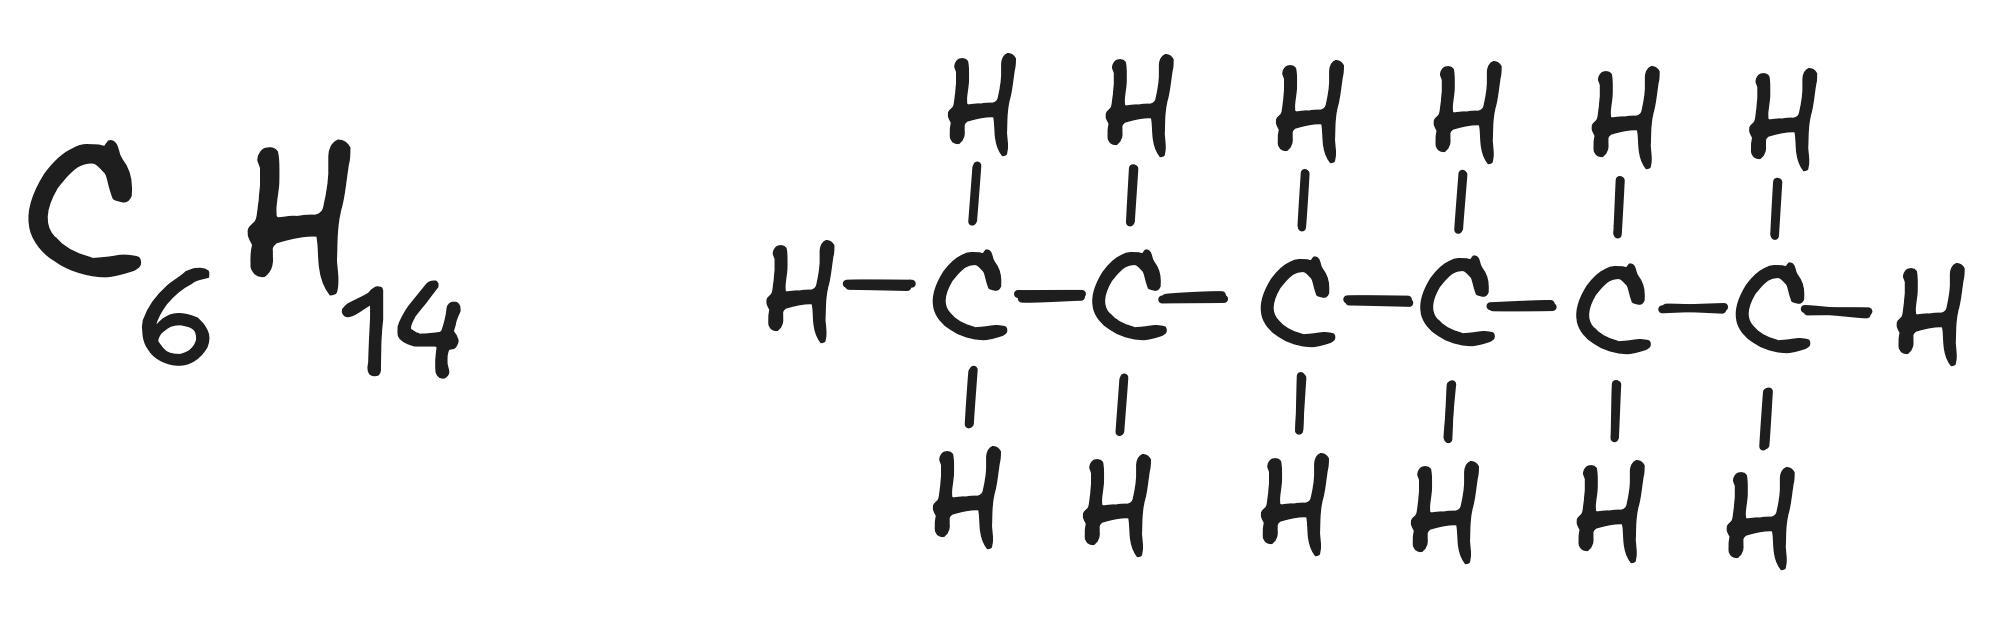
\includegraphics[width=0.4\textwidth]{hexan.png}
\end{figure}
\vspace{5mm}

\break

\question Vad skiljer stärkelse och cellulosa? Vart hittar vi dem och vilken av dem kan vi människor brytan ner? (\textbf{2 poäng})
\vspace{50mm}

\question Resonera kring varför vissa ämnen är miljögifter och hur de kan påverka levande organismer. (\textbf{2 poäng})
\vspace{50mm}

\question Förklara hur kolatomens egenskaper gör den speciell för livets kemi (organisk kemi). Använd relevanta begrepp och figurer.(\textbf{3 poäng})
\vspace{50mm}

\end{questions}

\end{document}
